\documentclass{report}

\usepackage{amsthm}
\usepackage{graphicx}
\usepackage{subcaption} 
\usepackage{color}


\setcounter{tocdepth}{0}

\newtheorem{definition}{Definition}

\newcounter{todoNoteCounter}
\newcommand{\todo}[1]{{\scriptsize  \color{red} \refstepcounter{todoNoteCounter}\textsf{[TODO]$_{\arabic{todoNoteCounter}}$:{#1}}}}

\newcommand{\vars}{V}
\newcommand{\init}{I}
\newcommand{\goal}{G}
\newcommand{\actions}{A}
\newcommand{\mutexes}{M}
\newcommand{\vals}{W}
\newcommand{\dom}[1]{dom(#1)}
\newcommand{\var}[1]{var(#1)}
\newcommand{\pre}[1]{pre(#1)}
\newcommand{\add}[1]{add(#1)}
\newcommand{\del}[1]{del(#1)}
\newcommand{\eff}[1]{eff(#1)}
\newcommand{\con}[1]{con(#1)}
\newcommand{\pro}[1]{pro(#1)}
\newcommand{\wan}[1]{wan(#1)}
\newcommand{\isAnyValue}[1]{isAnyValue(#1)}


\begin{document}
	
	%\chapter{PSM-SAS reduction planner}
	
	\tableofcontents
	
	\input{notation}
	
		\chapter{Merging values through small cycles -mv}
	
	Let assume that we have two facts $u_i, u_j$ and two actions. Each action has only one effect and zero prevail precondition. One action has got effect of type $<u_i,u_j>$ and the second one has got opposite effect to this one. So, we have two facts and can get from one to another by applying one of these actions. This is possible because the actions do not have any other side effect nor precondition. 
	
	The reduction works in the way that the two facts are merged to one. Such a reduction is very practical because it can reduce number of facts and also another reduction may arise.
	
	\begin{figure}
		\begin{subfigure}[b]{0.4\textwidth}
			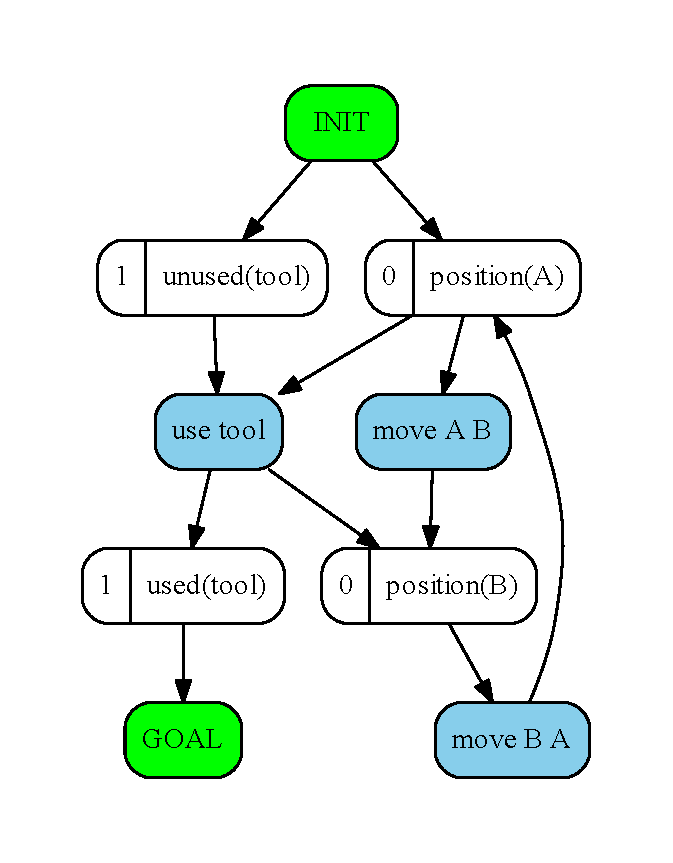
\includegraphics[scale=0.4]{mergingValues/figures/simple_input}
			\caption{before reduction}
		\end{subfigure}	
		\begin{subfigure}[b]{0.4\textwidth}
			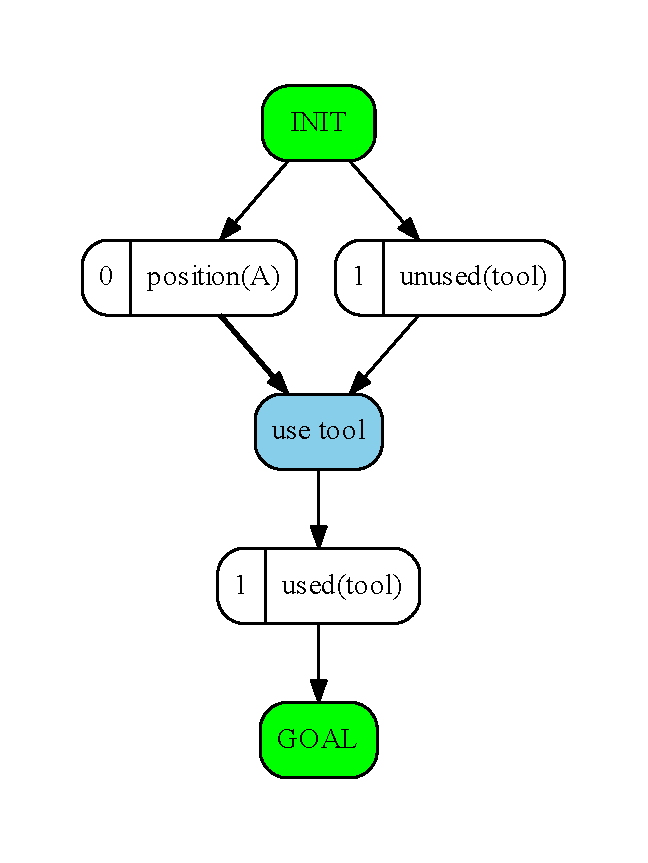
\includegraphics[scale=0.4]{mergingValues/figures/simple_output}
			\caption{after reduction}
		\end{subfigure}
		\caption{facts \emph{0 position(A)} and \emph{0 position(B)} can be merged because there are actions \emph{move A B} and \emph{move B A} switching from one fact to another without any other side effects nor preconditions}
	\end{figure}
	
	
	\section{Reduce operation}
	
	Let suppose that we have SAS in form of $<\vars, \init, \goal, \actions, \mutexes{}>$ and two actions $a_i, a_j \in \actions, a_i \neq a_j$. Operation of merging values will be done only if \ref{MSC:in:first}, \ref{MSC:in:second}, \ref{MSC:in:fourth:commonVariable} are satisfied and one of \ref{MSC:in:third:common}, \ref{MSC:in:third:2any}, \ref{MSC:in:third:1any} is satisfied.
	
	
	\begin{enumerate}
		\item $\pre{a_i} = \emptyset \land \pre{a_j} = \emptyset $ \label{MSC:in:first}
		\item $|\add{a_i}| = 1 \land |\add{a_j}| = 1 $ \label{MSC:in:second}
		\item let set $e_i \in \eff{a_i}$, $e_j \in \eff{a_j}$ and $v = \var{\add{e_i}}$
		\item $\var{\add{e_i}} = \var{\add{e_j}}$ \label{MSC:in:fourth:commonVariable}
		\item	\begin{enumerate}
			\item $\add{e_i} = \del{e_j} \land \add{e_j} = \del{e_i}$ \label{MSC:in:third:common}
			\item $\isAnyValue{\del{e_i}} \land \isAnyValue{\del{e_j}} $ \label{MSC:in:third:2any}
			\item $\isAnyValue{\del{e_i}} \land \add{e_i} = \del{e_j}$ \label{MSC:in:third:1any}
		\end{enumerate}
	\end{enumerate}
	
	Let set $u_i = \add{e_i}$ and $u_j = \add{e_j}$. This operation does following things: renames $u_j$ to $u_i$ in all occurrences in actions, mutexes, init and goal \ref{MSC:out:rename}. Then removing $u_j$ from the domain \ref{MSC:out:mergeValues}. Then effects of type $<u_i, u_i>$ are removed from operators \ref{MSC:out:changeOperators:3}. To each action, from which $<u_i, u_i>$ was removed, precondition $u_i$ is added \ref{MSC:out:addPre}. Then actions having zero effects are removed \ref{MSC:out:removeOperators}.
	
	Note that \ref{MSC:out:addPre} was added to the reduction after a bug appeared on some airport domain which was already reduced by generalize actions reduction. Adding such precondition ensures that extension operation will produce valid plan.
	
	\begin{enumerate}
		\item rename all occurrences in SAS of $u_j$ to $u_i$ \label{MSC:out:rename} \begin{enumerate}
			\item if $u_j \in \init$ then $\init{}' \leftarrow (\init \setminus \{u_j\}) \cup \{u_i\}$; else $\init{}' \leftarrow \init$
			\item if $u_j \in \goal$ then $\goal{}' \leftarrow (\goal \setminus \{u_j\}) \cup \{u_i\}$; else $\goal{}' \leftarrow \goal$
			\item $u_j$ is replaced by $u_i$ in all occurrences in $\pre{a}, \add{a}, \del{a} \forall a \in \actions$; store these actions to $\actions$
			\item $u_j$ is replaced by $u_i$ in each mutex where $u_j$ occurs; store final mutexes to $\mutexes{}'$
		\end{enumerate}	
		\item $\dom{v} := \dom{v} \setminus \{u_j\}$ \label{MSC:out:mergeValues}
		\item \begin{enumerate} 
			\item $A_c := \{a | a \in \actions, u_i \in (\del{\eff{a}} \cup \add{\eff{a}}) \}$ \label{MSC:out:changeOperators:1}
			\item remove all occurrences of effect of type $<u_i, u_i>$ in $A_c$ and store it to $A_d$ \label{MSC:out:changeOperators:2}
			\item $A_p \leftarrow \{<\pre{a} \cup \{u_i\},\eff{a}> | a \in A_d \}$ \label{MSC:out:addPre}
			\item set $A_d' := (\actions \setminus A_c) \cup A_p$ \label{MSC:out:changeOperators:3}
		\end{enumerate} 
		\item $\actions{}' := \{a | a \in A_d', \eff{a} \neq \emptyset \}$ \label{MSC:out:removeOperators}
	\end{enumerate}
	
	Afterwards, output SAS looks like $<\vars, \init{}', \goal{}', \actions{}', \mutexes{}'>$.
	
	Since we defined mutex as a set of values, so in case that $u_j$ is renamed to $u_i$ and both of them are in the same mutex, only $u_i$ remains in the mutex.
	
	
	\section{Possible outgoing states of SAS}
	
	Following states of SAS can appear after the reduction:
	
	\begin{itemize}
		\item $v$ has only one value in its domain (which can be removed by delete variable operation)
		\item mutex $m$ containing both $u_i$ and $u_j$ before the reduction, will contain only $u_i$ afterwards
		\item mutex $m$ containing $u_j$ but not $u_i$ before the reduction, will contain $u_i$ afterwards
% blbost, neni akce ktera by mela takovyhle efekty protoze by byla nesplnitelna
%		\item also note that actions has a set of effect, therefore if in step \ref{MSC:out:changeOperators:2} situation raises that $a_1$ has got effects $\{<u_n,u_j>, <u_n,u_i>\}$ and merging $u_i$ and $u_j$ is processed, after that effects of $a_1$ looks like $<u_n,u_i>$
		\item variable $v$ has at least one value
		\item after this operation a new situation in which -mv can be used may rise
	\end{itemize}
	
	
	\section{States before application of this operation}
	\begin{itemize}
		\item the original SAS
		\item after deleting variable 
		\item after another MV
	\end{itemize}
	
	
	
	\section{Reverse operation}
	
	While making this reduction, we remember $a_i$ and $a_j$. The reverse operation is done in following way:
	
	Firstly, $\dom{v} := \dom{v} \cup \{u_j\}$ and $u_i$ is renamed to $u_j$ at places (mutex, init, goal, effects, preconditions, etc) where $u_j$ was used before the merge operation.
	
	Secondly, removed operators from step \ref{MSC:out:changeOperators:3} are added and also the removed effect are added. Prevail preconditions that were added during reduction are removed.
	
	Then, to $s$ value of initial value of variable $v$ is loaded. The produced plan is then traversed, action by action. If traversed action $a$ has got $v$ in its precondition (either prevail or precondition of unconditional effect), following procedure is applied:
	
	In the case that $a$ needs $u_j$ and value $u_i$ is in $s$ then action $a_j$ is added to plan before $a$. Similar case is when $u_i$ and $u_j$ are switched, then $a_i$ is added to plan before $a$.
	
	In the case that $a$ needs $u_j$ and value $u_j$ is in $s$ then nothing is done; similar when this situation raises with value $u_i$.
	
	After each application of an action $a$ from the plan that effects variable $v$, value of $s$ is updated.
	
	Finally, after processing all actions of the plan, value in $s$ is compared with value of variable $v$ in $\goal$ and the plan is expanded by the previous method if it needs to be. The extended plan is returned as output of the reverse action.
	
	
	\section{Implementation notes}
	In implementation, while merging $u_j$ and $u_i$, value with bigger id is selected to be replaced by the other.
	
	Also, FD crashes when having a variable with only one value, therefore operation of deleting variables has to be run before running FD.
	
	
		\chapter{Big merging values through small cycles -bv}
	
	Another implementation of -mv. The difference is that this operation does more -mv operations in one steps. Extending of the plan is done by extending given plan by reverse operations in the spite of -mv that are processed in reversed order than reductions were made.
	
	\section{Implementation notes}
	Note that the implementation may need two calls to example such there are actions $a_1:0 \rightarrow 1$, $a_2:1 \rightarrow 0$, $a_3:1 \rightarrow 2$, $a_4:2 \rightarrow 0$ (actions switch the same variable, no preconditions). The implementation will return only one reverse operation of -bv if the actions will be processed in sequences like $a_1, a_2, a_3, a_4$ or $a_2, a_1, a_4, a_3$, etc. But in case that the actions will be processed in sequences like $a_3, a_4, a_1, a2$ or $a_4, a_3, a_2, a1$, etc., there will be two -bv reverse operation returned because it does when merging $a_1$ and $a_2$ it does not further look to the memory if stored actions (that happens in the second case) can be merged.
	
	
	
	
	\chapter{Delete variable -dv}
	
	If there is variable having only one value, then such a variable can be removed from the problem because it becomes redundant. It is redundant since init sets the variable to its only value and the variable cannot be changed to any other value. Note that the variable can appear only in prevail preconditions. 
	
	\begin{figure}
		\begin{subfigure}[b]{0.4\textwidth}
			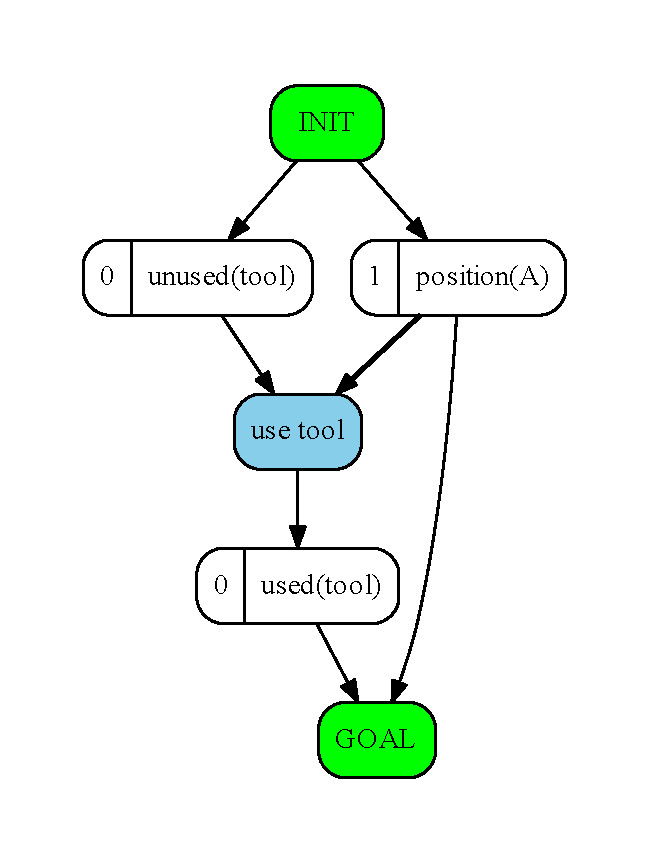
\includegraphics[scale=0.4]{deleteVariable/figures/simple_input}
			\caption{before reduction}
		\end{subfigure}	
		\begin{subfigure}[b]{0.4\textwidth}
			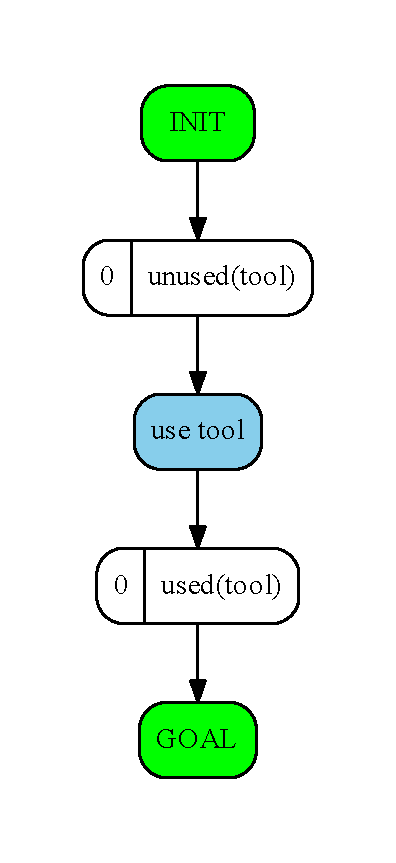
\includegraphics[scale=0.4]{deleteVariable/figures/simple_output}
			\caption{after reduction}
		\end{subfigure}
		\caption{variable 1 can be removed because it becomes redundant as can be seen}
	\end{figure}
	
	
	\section{Reduce operation}
	Let have SAS in form $<\vars, \init, \goal, \actions, \mutexes{}>$. This reduction is performed if there is $v \in \vars: |\dom{v}| = 1$. Let work with such variable $v$.
	
	Let $u$ be the only remaining value of variable $v$. The reduction operation performs following steps: removing $v$ from variables \ref{RV:out:remove}, removing preconditions with $v$ \ref{RV:out:act} (we assume that there are no effects of type $<e,e>$ where $e \in \dom{v}$), removing the value from init \ref{RV:out:init}, goal \ref{RV:out:goal} and mutexes \ref{RV:out:mutex}.
	
	\begin{enumerate}
		\item $\vars{}' \leftarrow \vars \setminus \{v\}$ \label{RV:out:remove}
		\item $\init{}' \leftarrow \init \setminus \{u\}$ \label{RV:out:init}
		\item $\goal{}' \leftarrow \goal \setminus \{u\}$ \label{RV:out:goal}
		\item \begin{enumerate}
			\item $\actions{}_c \leftarrow \{a | a \in \actions, u \in \pre{a}\}$
			\item remove preconditions containing value $u$ from $\actions{}_c$ and store these actions to $\actions{}_d$
			\item $\actions{}' \leftarrow (\actions \setminus \actions{}_c) \cup \actions{}_d$ \label{RV:out:act}
		\end{enumerate}
		\item remove value $u$ from all mutexes and store that with unchanged mutexes to $\mutexes{}'$ \label{RV:out:mutex}
	\end{enumerate}
	
	Output of the reduction is SAS $<\vars{}', \init{}', \goal{}', \actions{}', \mutexes{}'>$.
	
	\section{Possible outgoing states of SAS}
	Following states of SAS can occur after the reduction:
	
	\begin{enumerate}
		\item mutex may be empty after this operation 
		\item state where -mv can be applied may be made
		\item some actions may have fewer preconditions, therefore some actions may be merged together as similar
		\item state where simple dependency may be applied may be made
	\end{enumerate}
	
	\section{States before application of this action}
	\begin{itemize}
		\item -mv can caused this
		\item removing some value, therefore after application of dead ends, one effect reduction or using pruning by -uv
	\end{itemize}
	
	
	\section{Reverse operation}
	The reverse operation is quite simple. The things that were removed during reduction, are added back to the SAS (at all places - in mutexes, operations, init, goal and variables).
	
	
	\section{Implementation notes}
	This operation needs to be run as last one to ensure that FD will not crash.
	
	
	
	
	
	
	\chapter{Simple dependency -sd}
	Let assume that there is a fact such that, there is only one action producing this fact and only one action deleting this fact (there is no action that has got this fact in prevail precondition). Then it may seem reasonable to merge both actions to only one instead to lower number of actions. 
	
	This operation does such a merging of actions, but the thing is not so trivial as it may seem. To merge both actions they have to be \emph{atomic}. In short it means that if action adding the fact is applied, then the second action can be applied as well. 
	
	\begin{figure}
		\begin{subfigure}[b]{0.4\textwidth}
			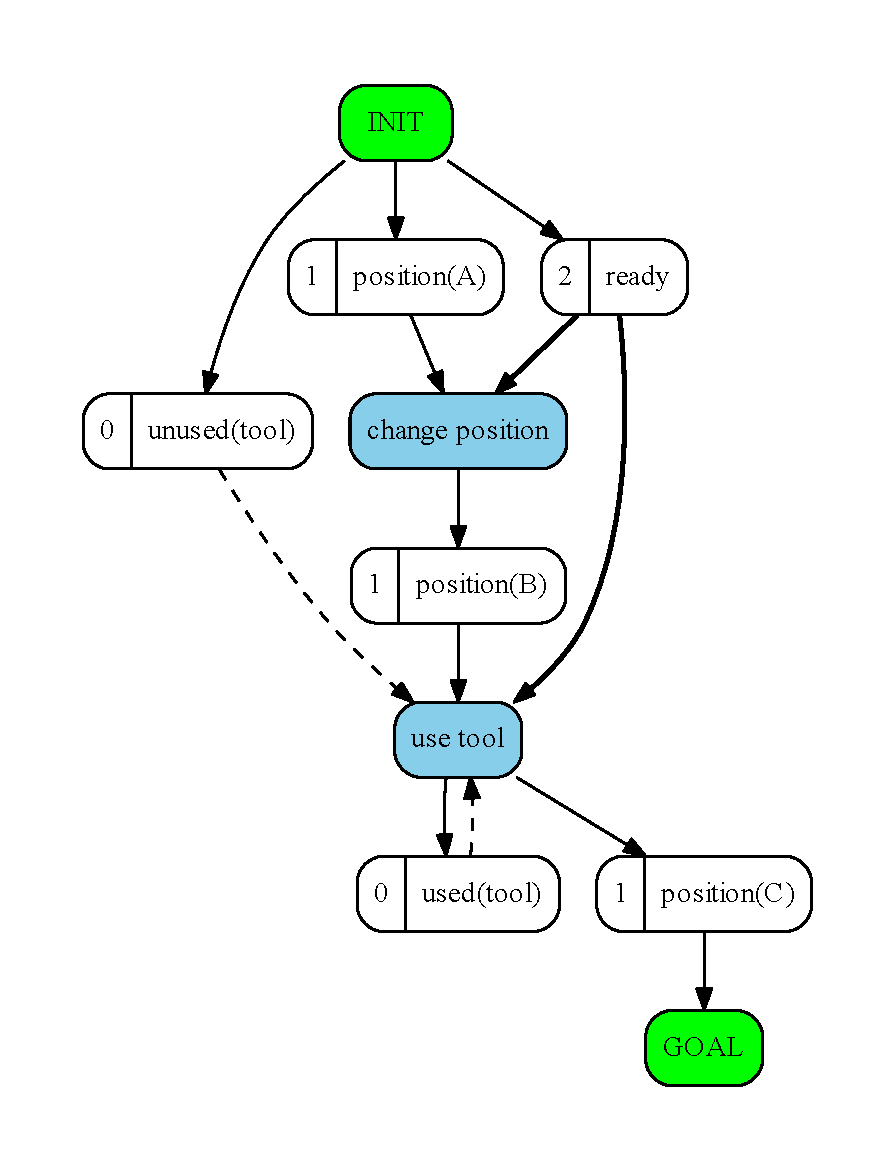
\includegraphics[scale=0.4]{simpleDependency/figures/simple_input}
			\caption{before reduction}
		\end{subfigure}	
		\begin{subfigure}[b]{0.4\textwidth}
			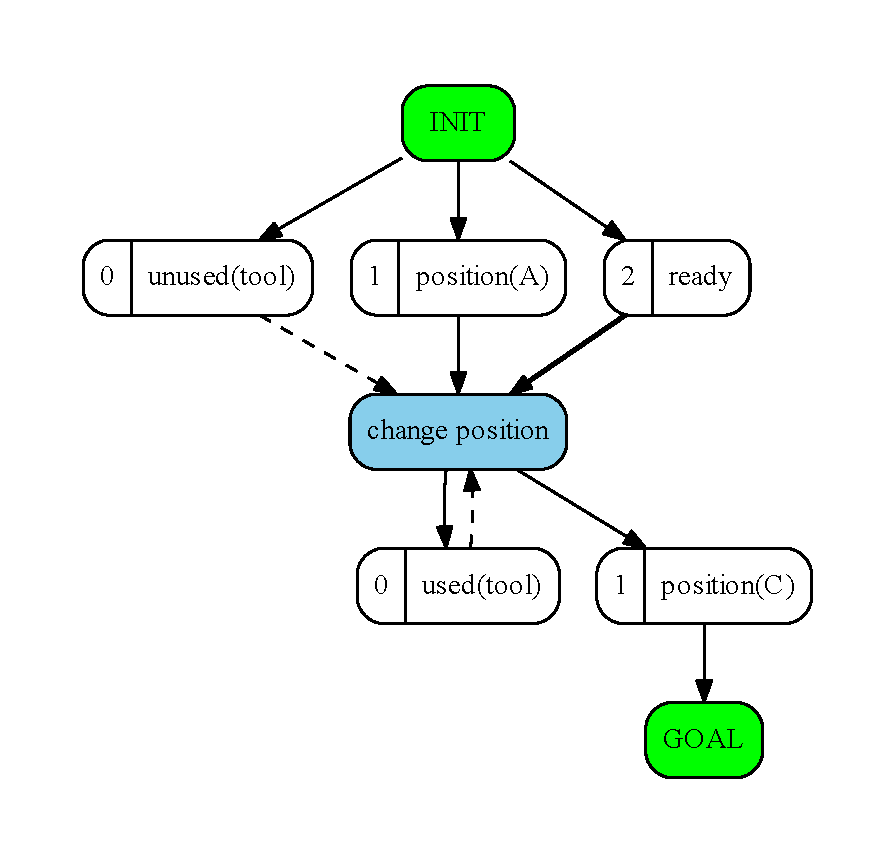
\includegraphics[scale=0.4]{simpleDependency/figures/simple_output}
			\caption{after reduction}
		\end{subfigure}
		\caption{actions \emph{change position} and \emph{use tool} can be merged to one}		
	\end{figure}
	
	\section{Reduce operation}
	Lets have SAS in form $<\vars, \init, \goal, \actions, \mutexes{}>$. This operation will be executed if the following will hold:
	
	\begin{enumerate}
		\item there is a value $u$, which is not in init and not in goal; $u \notin \init$, $u \notin \goal$
		\item only one action $a_i$ that adds $u$; $|\{a | a \in \actions, u \in \add{a}\}| = 1$
		\item $a_i$ adds only $u$; $\add{a_i} = \{u\}$
		\item only one action $a_j$ that needs $u$; $|\{a | a \in \actions, u \in \pre{a} \lor u \in \del{a} \}| = 1$
		\item to ensure atomicity there must hold that $\pre{a_i} \subseteq \pre{a_j}$
		\item if there is a effect in $\eff{a_j}$ of type $<-1,w>$, then any value of $\var{w}$ must not be in $\pre{a_i}$
	\end{enumerate}
	
	We assume that if a value is in $del$ of a operator, then the value is not present in the operator's $pre$. Now, the reduction is following:
	
	\begin{enumerate}
		\item $\dom{v} := \dom{v} \setminus \{u\}$ 
		\item $u$ is also removed from mutexes as in -dv; final mutexes are stored to $\mutexes{}'$
		\item if $u \in \pre{a_j}$ then $p \leftarrow (\pre{a_i} \cup \pre{a_j}) \setminus \{u\}$, $e \leftarrow <\del{a_i} \cup \del{a_j}, \add{a_i} \cup \add{a_j}>$ \label{SD:out:wrong}
		\item if $u \in \del{a_j}$ then set $u_p : <u_p, u> \in \eff{a_i}, u_n : <u, u_n> \in \eff{a_j}$ $p \leftarrow \pre{a_i} \cup \pre{a_j}$, $e \leftarrow <(\del{a_i} \cup \del{a_j}) \setminus \{u\}, (\add{a_i} \cup \add{a_j}) \setminus \{u\}>$, so instead of two effect $<u_p, u>, <u, u_n>$ there is only one $<u_p, u_n>$ \label{SD:out:inEffect}
		\item $a_n \leftarrow <p,e>$
		\item $\actions{}' \leftarrow (\actions \setminus \{a_i, a_j\}) \cup \{a_n\}$		
	\end{enumerate}
	
	Output of the reduction is SAS $<\vars{}, \init{}, \goal{}, \actions{}', \mutexes{}'>$.
	
	
	\textbf{There is a mistake:} this procedure is implemented in the code but it does not follow the difference of $u$ being in prevail precondition and delete of an action right. If $u$ is in delete effect of $a_j$, then it will work fine. But if $u$ is in prevail precondition of $a_j$, then by merging $a_i$ with $a_j$ we get new action that is possible to be applicable only once. But there is possibility that $a_i$ adds $u$ but $a_j$ can be executed multiple times. For example, $a_j = <\{u\}, <-1,v>>$ where $v$ is value such that $\var{u} \neq \var{v}$. In such case no merging is possible; therefore \ref{SD:out:wrong} is wrong behavior and $u$ should be only in $\del{a_i}$.
	
	\section{Possible outgoing states of SAS}
	\begin{enumerate}
		\item state where -mv is applicable may happen
		\item another -sd may appear
	\end{enumerate}
	
	\section{States before application of this action}
	\begin{itemize}
		\item after -mv
		\item after merging of similar actions -mo
		\item after -dv
	\end{itemize}
	
	
	\section{Reverse operation}
	In the reverse operation, $a_n$ is removed from $\actions$ and $a_i$ and $a_j$ are added back to $\actions$. Moreover, other things done during reduction are reverted.
	
	Procedure of extending plan is quite simple. The plan is traversed action by action. When there there is action $a_n$ in the plan, it is replaced by sequence of actions $(a_i, a_j)$ at the same place. Extended plan is returned.
	
	
	\section{Implementation notes}
%	Possible natural but not implemented extension of this reduction is to use goal and init as special action and use simple dependency with them. But it would work only if init would add one value only or goal contains only one value.

	Possible natural extension of this operation is to do merging not only over value $u$ but over set of values (one action adds more values that only another action needs).	
	
	This is little bit awful, but this is the only operation that in fact adds something to an action. Therefore this updated action has to be cached in SasFile class. But the caching is there only because of speedup (we do not want to traverse all operators all the tame).
	
	
	\chapter{Merging similar operators -mo}
	
	Let assume that we have two or more actions that are similar (\ref{notation:similarActions}). In such case we can select only one action and the rest remove. This is because rest of the actions become redundant. By this, number of action is decreased and some other reduction may start to work because we get rid of multiple possibilities how to add some fact (some reductions need to know that the fact is added only by one action, etc).
	
	\begin{figure}
		\begin{subfigure}[b]{0.4\textwidth}
			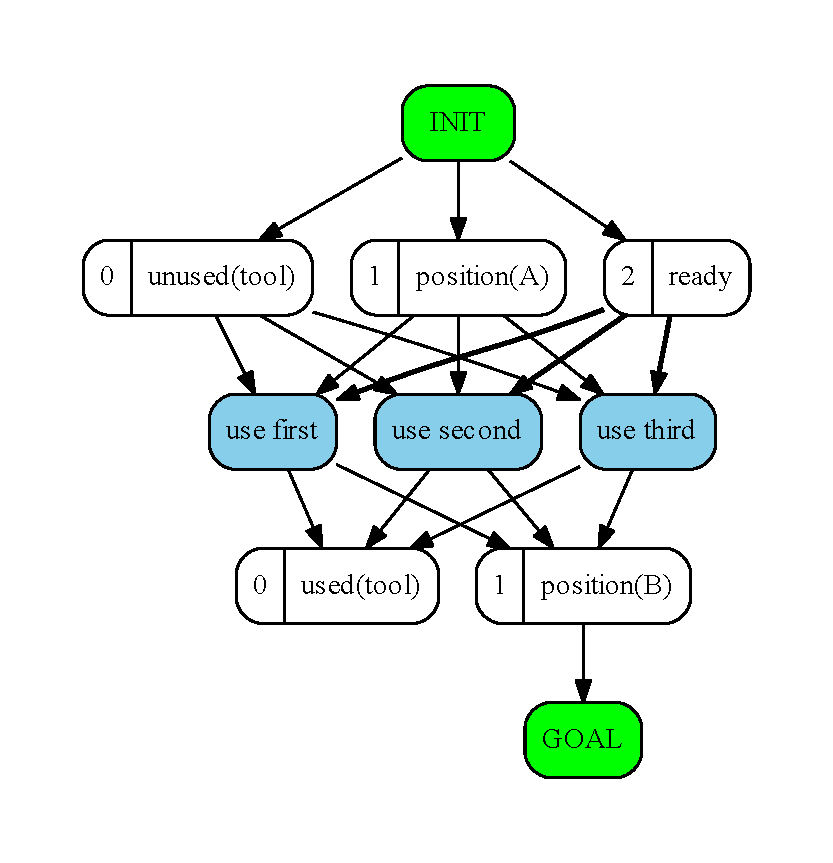
\includegraphics[scale=0.4]{mergingSimilarOperators/figures/threeToOne_input}
			\caption{before reduction}
		\end{subfigure}	
		\begin{subfigure}[b]{0.4\textwidth}
			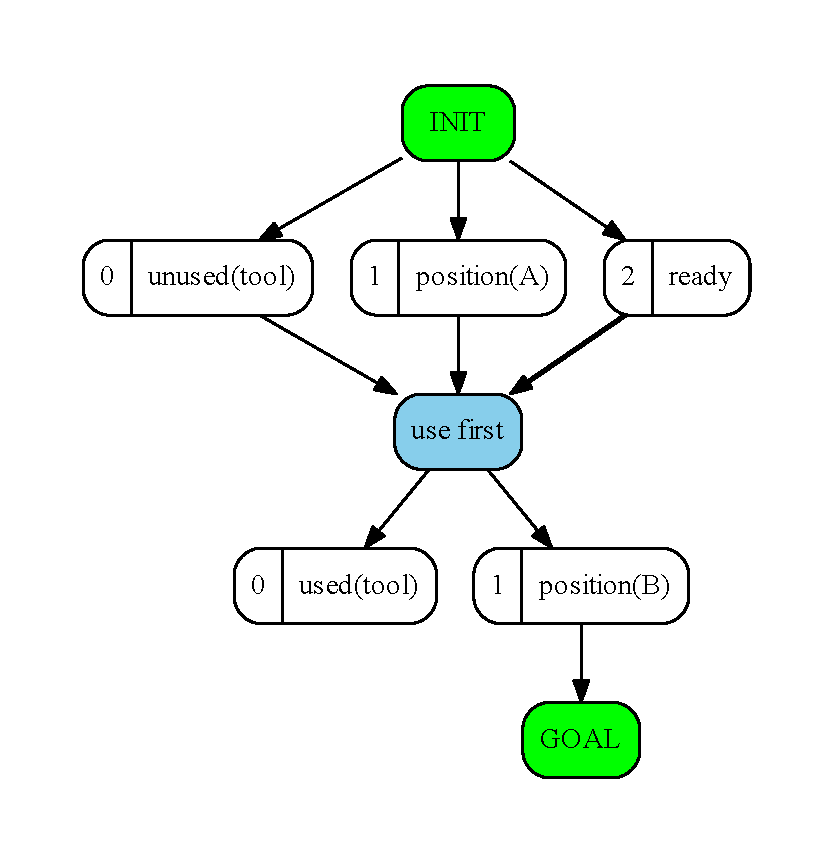
\includegraphics[scale=0.4]{mergingSimilarOperators/figures/threeToOne_output}
			\caption{after reduction}
		\end{subfigure}
		\caption{All of the action in the example can be removed, but one representative of these action has te be preserved in the instance.}		
	\end{figure}	
	
	
	\section{Reduce operation}
	Let's have SAS in form $<\vars, \init, \goal, \actions, \mutexes{}>$. The following reductions is executed only if there is a set of similar actions that has got more than one action. Let have such a set $\actions{}_s$.
	
	The reduction does following things: pick arbitrary action $a \in \actions{}_s$. Remove all actions from $\actions{}$ each action in $\actions{}_s$ but not $a$; $\actions{}' \leftarrow (\actions \setminus \actions{}_s) \cup \{a\}$.
	
	Output of the reduction is SAS $<\vars{}, \init{}, \goal{}, \actions{}', \mutexes{}>$.
	
	\section{Possible outgoing states of SAS}
	\begin{enumerate}
		\item possible state of SAS for application of -sd
	\end{enumerate}
	
	\section{States before application of this operation}
	\begin{itemize}
		\item original SAS
		\item after -dv, -mv, -oe
	\end{itemize}
	
	
	\section{Reverse operation}
	Since the actions have got same effects and preconditions, only $a$ is allowed to be used in the plan. Moreover, no extending of the plan is done. This comes from the fact that we think that if two actions are similar, then they were either similar from the start or they got similar during reductions. If they got similar during reductions, then we can get by application of reverse operators from one action to another (in the similar set), eg. to get to state where any of the action from the $\actions{}_s$ is applicable. But this is rather unproven idea.
	
	\section{Implementation notes}
	There could be (but is not implemented) filter for deleting similar actions while parsing. Because then we would have the information whether the actions were similar from the beginning or if they become similar during reductions.
	
	
	
	
	
		
	\chapter{Pruning unreachable values -uv}
	
	This reduction does delete relaxation to test whether some each fact is reachable and each operation is applicable. If a fact or operation is not reachable nor applicable in the delete relaxation, then it cannot be used in plan without delete relaxation neither with it. Therefore such facts and operations can be removed. 
	
	\begin{figure}
		\begin{subfigure}[b]{0.4\textwidth}
			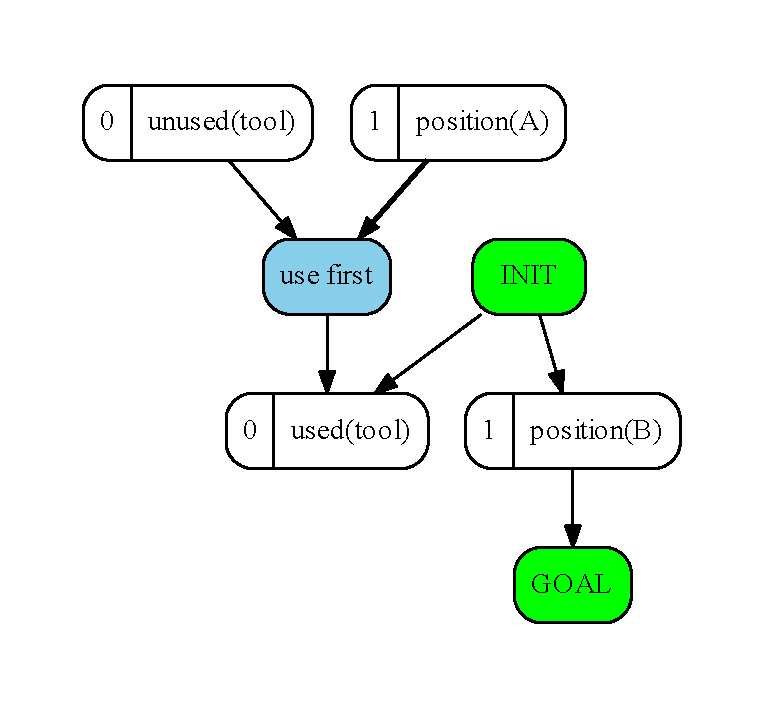
\includegraphics[scale=0.4]{unreachableValues/figures/simple_input}
			\caption{before reduction}
		\end{subfigure}	
		\begin{subfigure}[b]{0.4\textwidth}
			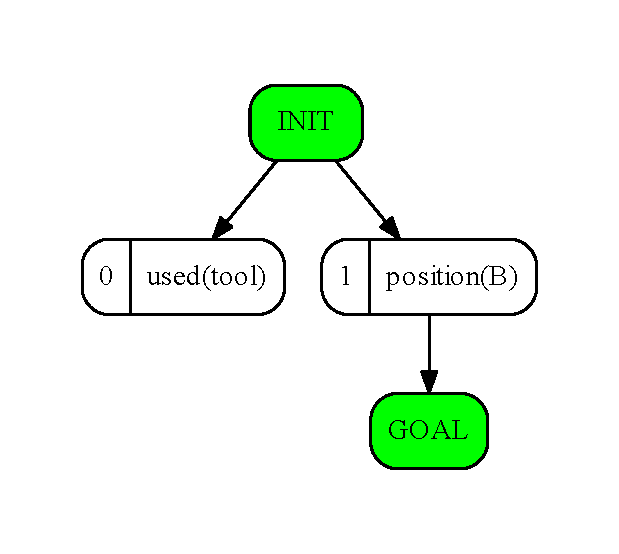
\includegraphics[scale=0.4]{unreachableValues/figures/simple_output}
			\caption{after reduction}
		\end{subfigure}
		\caption{Facts \emph{0 unused(tool)} is unreachable, therefore action \emph{use first} is not applicable. Fact \emph{1 position(A)} is unreachable as well. So these facts and action can be removed. }
	\end{figure}
	
	\section{Reduce operation}
	Let's have SAS in form $<\vars, \init, \goal, \actions, \mutexes{}>$.  Firstly, this operation does delete relaxation by DFS search. The DFS firstly marks all values form $\init$ as reachable and then applies each applicable action and marks its values from $add$ as reachable. Moreover it removes the applied action from the set of action over which it iterates (it is filled by $\actions$ in the beginning). This procedure iterates untill there are no applicable action in the set . After DFS is processed, it has got two sets; set of unreachable values $\vals{}_u$ and set of unreachable actions $\actions{}_u$. Note, that in $\vals{}_u$ there is no value from $\init$. Now, the reduction does following things:
	
	\begin{enumerate}
		\item for each $u \in \vals{}_u$: $u$ is removed from domains ($\vars{}'$ contains variable after this operatiron)
		\item each $u \in  \vals{}_u$ is removed from mutexes ($\mutexes{}'$ contains mutexes after this operation)
		\item $\actions{}' \leftarrow \actions \setminus \actions{}_u$
	\end{enumerate}
	
	Output of the reduction is SAS $<\vars{}', \init{}, \goal{}, \actions{}', \mutexes{}'>$.
	
	\section{Possible outgoing states of SAS}
	\begin{enumerate}
		\item mutex may be empty after this operation
		\item check for removing value from $\goal$ is not implemented, since we assume only plannable instances
		\item possible states of SAS for application of delete variable -dv or merging operators -mo
	\end{enumerate}
	
	\section{States before application of this operation}
	\begin{itemize}
		\item SAS from the beginning
		\item when an effect is removed from action and the value that is added by the effect is not removed (implementation note)
	\end{itemize}
	
	\section{Reverse operation}
	During reverse operation, $\actions{}_u$ are added back to $\actions$ and $\vals{}_u$ are added back to $\vals$ and $\mutexes$.
	
	\section{Implementation notes}
	While removing operators we assume that all operators were active before calling -uv. 
	
	
	
	
	\chapter{Dead ends -de}

	Suppose that you know that some fact does not appear in any precondition nor delete effect of any action; also the fact is not in init nor goal. Then there are two possibilities, either it has the function that the action adding the fact may be used at most once (the action has another effect); or it is dead end (it is redundant). Such dead end facts can be removed together with actions that produce them.
	
	This operation does precisely this thing; it removes such redundant facts and actions
	
	\begin{figure}
		\begin{subfigure}[b]{0.4\textwidth}
			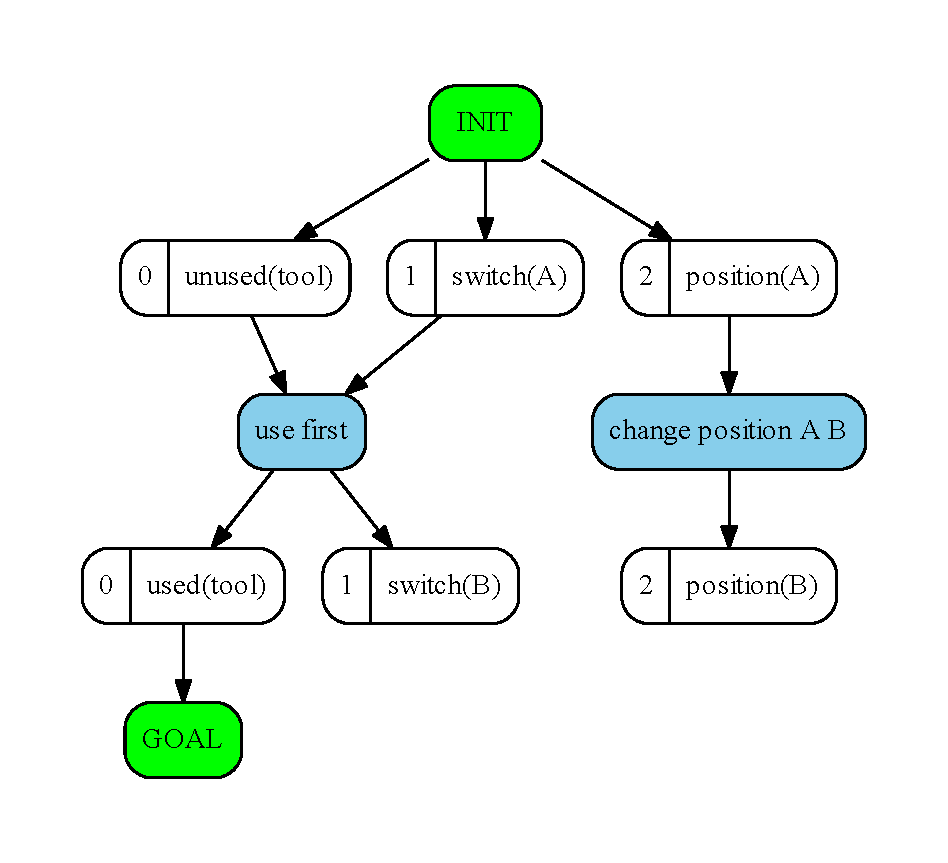
\includegraphics[scale=0.35]{deadEnds/figures/oneDeadEnd_input}
			\caption{before reduction}
		\end{subfigure}	
		\begin{subfigure}[b]{0.4\textwidth}
			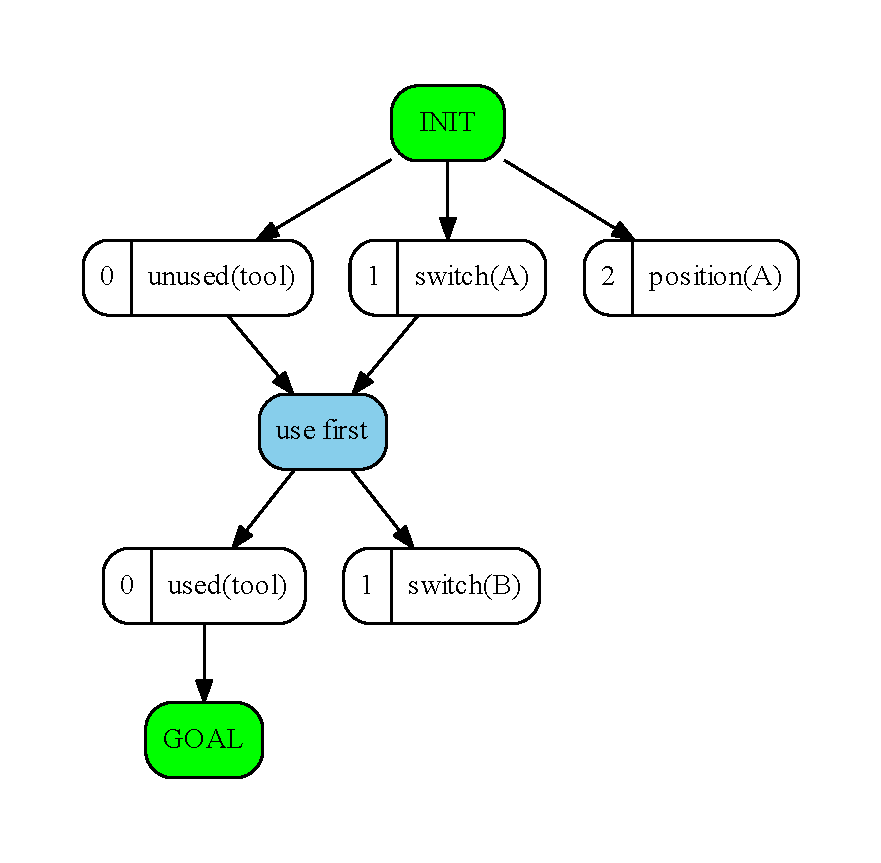
\includegraphics[scale=0.35]{deadEnds/figures/oneDeadEnd_output}
			\caption{after reduction}
		\end{subfigure}
		\caption{In this example fact \emph{2 position(A)} and action \emph{change position A B} may be removed because they are redundant. But fact \emph{switch(B)} cannot be removed because action \emph{use first} has more than one effect. }
	\end{figure}

	
	\section{Reduce operation}
	Let's have SAS in form $<\vars, \init, \goal, \actions, \mutexes{}>$. If there is a value $u$ such that:
	
	\begin{enumerate}
		\item $u \notin \init, u \notin \goal$
		\item $|\con{u}| =  0$
		\item there is no effect of type $<-1,u_i>, u_i \in \dom{\var{u}}$ in any $\actions{}$
		\item each action adding $u$ has only one effect; $1 = |\eff{a}| \forall a \in \pro{u}$	\label{de:in:invariants}
	\end{enumerate}

	Condition \ref{de:in:invariants} ensures that invariant won't be destroyed. If such condition would not be met, then delete relaxation could rise.

	Then the operation is executed. The operation does following things:
	
	\begin{enumerate}
		\item remove $u$ from domain of $\var{u}$
		\item remove $u$ from mutexes
		\item remove actions with zero effects
	\end{enumerate}
	
	Output of the reduction is SAS $<\vars{}', \init{}, \goal{}, \actions{}', \mutexes{}'>$.
	
	
	\section{Possible outgoing states of SAS}
	\begin{enumerate}
		\item possible empty mutex
		\item possible state of SAS for application DV
	\end{enumerate}

	\section{States before application of this operation}
	\begin{itemize}
		\item SAS from the beginning
		\item does not know any operation that could cause such state, so what about running dv only once to save time?
	\end{itemize}

	
	\section{Reverse operation}
	The reverse operation adds removed values and actions. No extending of plan is done.
	
	\section{Implementation notes}
	The operation is implemented in the way that it iteratively remove dead ends (values and actions) from the SAS untill there are any. Because by removing an value, actions that add that value are redundant and so on.
	
	
	
	
	
	
	\chapter{Half cycle -hc}
	Suppose that there are two facts $u_i, u_j$ and action with only one effect $<u_i,u_j>$ and no precondition. Then, if there is no other producer of $u_j$, nor any other action that needs $u_i$, $u_i$ is not in init and $u_j$ is not in goal, then whenever when $u_i$ is added, the only possible way to add $u_j$ is to use the action. Therefore we replace $u_j$ by $u_i$, remember that information and use it while expanding plan.
	
	Note that there must not be opposite effect ($<u_j,u_i>$) in any other action \todo{Where is this in specification?}. In such situation -mv can be executed.

	\begin{figure}
		\begin{subfigure}[b]{0.4\textwidth}
			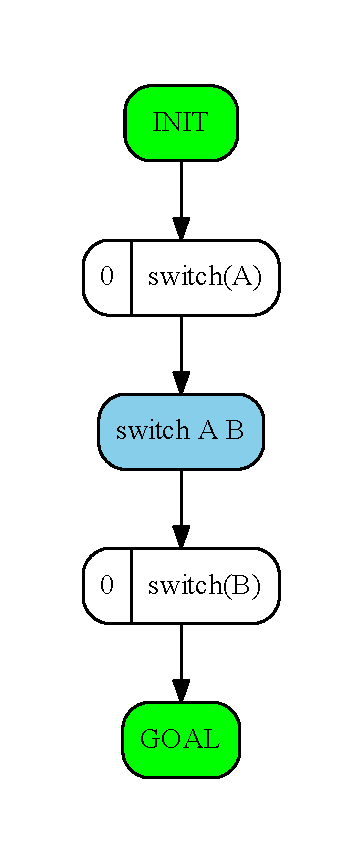
\includegraphics[scale=0.4]{halfCycle/figures/simple_input}
			\caption{before reduction}
		\end{subfigure}	
		\begin{subfigure}[b]{0.4\textwidth}
			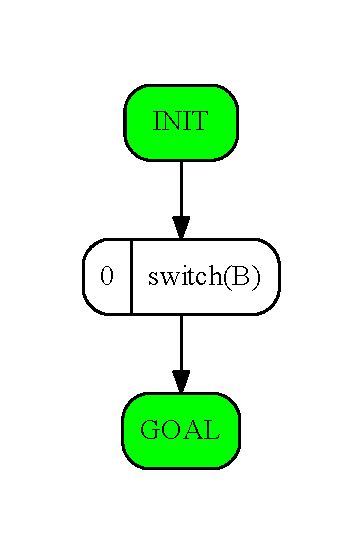
\includegraphics[scale=0.4]{halfCycle/figures/simple_output}
			\caption{after reduction}
		\end{subfigure}
		\caption{Example where facts \emph{0 switched(A)} and \emph{0 switched(B)} can be merged together because there is action \emph{switch A B} meeting all conditions for -hc reduction. }
	\end{figure}


	\section{Reduce operation}
	Let's have SAS in form $<\vars, \init, \goal, \actions, \mutexes{}>$. 
	
	In order to execute this operation there must be values $u_i, u_j$ and action $a$ such that:
	
	\begin{enumerate}
		\item $\var{u_i} = \var{u_j}$
		\item $u_j \notin \init$ \todo{why?}
		\item $u_i \notin \goal$ \todo{why?}
		\item $<u_i,u_j> \in \eff{a}$
		\item $|\eff{a}| = 1$
		\item $|\pre{a}| = 0$
		\item $\con{u_i} = 1$
		\item $\pro{u_j} = 1$ \todo{not necessary}
	\end{enumerate}
	
	The operation does following things:
	
	\begin{enumerate}
		\item replace $u_j$ by $u_i$ in actions and mutexes, and in goal if needs be
		\item remove $u_j$ from $\dom{\var{u_j}}$		
	\end{enumerate}
	
	Output of the reduction is SAS $<\vars{}', \init{}, \goal{}, \actions{}', \mutexes{}'>$.
	
	
	\section{Possible outgoing states of SAS}
	\begin{enumerate}
		\item -mv, -mo, maybe -sd and some other
	\end{enumerate}
	
	\section{States before application of this operation}
	\begin{itemize}
		\item from the beginning
		\item after -mo, -mv, -dv
	\end{itemize}
	
	
	\section{Reverse operation}
	Removed action is added back to SAS. While extending the plan, the plan is traversed and simulated. If $\var{u_i}$ is in state $u_i$ and the next operation needs $u_j$, then $a$ is added to the plan. Extended plan is returned.
	
	\section{Implementation notes}
	Simple implementation without any caching. Possible extension of this operation to search not action that works with 
	
	
	
	
	
		\chapter{One effect deletion -oe}
	
	This reduction is aimed to remove redundant invariants from operations. Firstly, action having effect of type $<u_i,u_j>$ ($u_i$ is not -1) can be used at most once in case that there is no action consuming $u_j$ ($|\con{u_j}| = 0$). Also, action can be used at most once if $|\pro{u_i}| = 0$, because there is no action producing $u_i$. 
	
	When there is an action that have two or more effect while one effect is $<u_i,u_j>$, the second $<w_i,w_j>$, ($u_i \neq -1, w_i \neq -1$) and following condition holds: $|\con{w_j}| = 0$, $|\pro{u_i}| = 0$. Then there is redundant invariant $<w_i,w_j>$. We already know that the action can be applied at most once, by deduction from $|\pro{u_i}| = 0$; therefore the invariant made by effect $<w_i,w_j>$ becomes redundant.
	
	Such redundant effect can be removed in case that there is no other action having $w_i$ in delete effect or prevail precondition; delete relaxation could rise without this condition. 
	
	\begin{figure}
		\begin{subfigure}[b]{0.4\textwidth}
			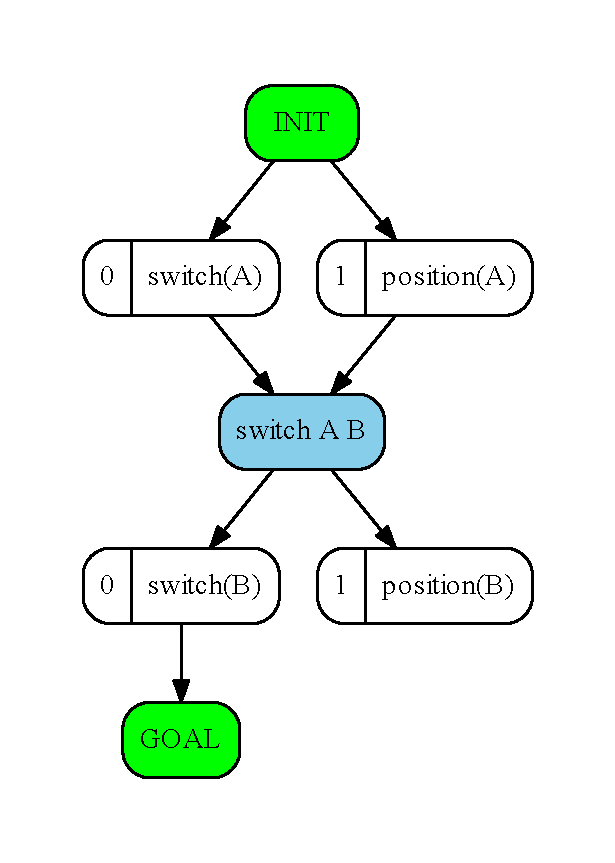
\includegraphics[scale=0.4]{oneEffectDelete/figures/simple_input}
			\caption{before reduction}
		\end{subfigure}	
		\begin{subfigure}[b]{0.4\textwidth}
			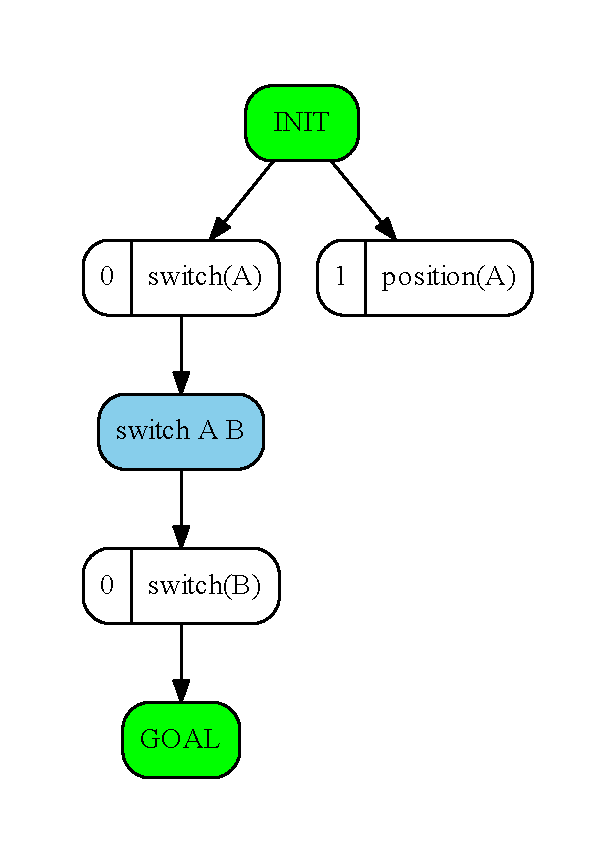
\includegraphics[scale=0.4]{oneEffectDelete/figures/simple_output}
		\caption{after reduction}
		\end{subfigure}
		\caption{Effect $<\emph{position(A)},\emph{position(B)}>$ can be removed from action \emph{switch A B} because effect $<\emph{switch(A)},\emph{switchtch(B)}>$ ensures that the action can be used at most once.}
	\end{figure}               
	
	
	
	\section{Reduce operation}
	Let's have SAS in form $<\vars, \init, \goal, \actions, \mutexes{}>$. There must be following values and actions in order to execute the action:
	
	\begin{enumerate}
		\item any value of variable $\var{u_i}$ is not in goal
		\item $u_i \in \init$
		\item $|\wan{u_i}| = 1$
		\item $|\pro{u_i}| = 0$
		\item $a \in \con{u_i}$
		\item $<u_i,u_j> \in \eff{a}$
		\item $|\con{u_j}| = 0$
		\item $<w_i,w_j> \ in \eff{a}, \var{w_i} \neq \var{v_i}$; action $a$ has another effect than $<u_i,u_j>$
		\item $|\con{w_j}| > 0$
		\item $|\pro{w_i}| = 0$
		\item $w_i \in \init$
	\end{enumerate}
	
	Action $a$ can be used only once, due to $<u_i, u_j>$. If there is another effect ($<w_i,w_j>$) that can be used only once, and its output ($w_j$) is used than the first effect can be omitted, because $u_j$ is not used in any other action. Also, there does not have to be any other action consuming $u_i$ or having it in prevail preconditon because of delete relaxation.
	
	
	The operation does following things:
	
	\begin{enumerate}
		\item $u_j$ is removed from $\dom{\var{u_j}}$
		\item $a_n \leftarrow <\pre{a}, \eff{a} \setminus \{<u_i,u_j>\}>$
		\item $\actions{}' \leftarrow (\actions \setminus \{a\}) \cup \{a_n\}$
	\end{enumerate}
	
	Output of the reduction is SAS $<\vars{}', \init{}, \goal{}, \actions{}', \mutexes{}>$.
	
	
	\section{Possible outgoing states of SAS}
	\begin{enumerate}
		\item states of SAS where -hc, -sd, -mo, -dv can be executed
	\end{enumerate}
	
	\section{States before application of this operation}
	\begin{itemize}
		\item original SAS
		\item after -ou, -mo, -dv, maybe others (-de)
		\item It seems that this operation is no longer needed when using -sf and -ai reductions, is it?
	\end{itemize}
	
	
	\section{Reverse operation}
	$a_n$ is removed from actions and $a$ is added back to the action set. Also, all occurrences of $a_n$ in plan are replaced by $a$.
		
	\section{Implementation notes}
	Simple implementation so far. There could be extension where $\var{u_i}$ is removed completely from the SAS (also actions that using $\var{u_i}$). It would be also faster.
	
	
	
	
	
	
	\chapter{One usage -ou}
	
	Having know that one action can be applied at most once is useful information in some cases. Let say that there is an action $a_c$ with effect $<w_i,w_j>$, no other action needs $w_i$ and there are also at least one action action having opposite effect ($<w_j,w_i>$). In such case, an cycle composed from facts $w_i$, $w_j$ and those actions is created. Now, our aim is to destroy such a cycle because it can further simplify the problem or another reduction may be applied. 
	
	The reduction itself is based on adding one new fact $w_n$ instead of $w_i$ or $w_j$ in one of the effects; so, either $<w_i,w_j>$ is replaced by $<w_i,w_n>$ or $<w_j,w_i>$ is replaced by $<w_j,w_n>$. The procedure when $w_i$ or $w_j$ is replaced is described further in reduction description.
	
	While doing this reduction, two things should be taken in mind. Firstly, effect cannot be removed from action and replaced by prevail precondition, since delete relaxation could occur; this may for example happen when there are multiple actions having the opposite effect to $a_c$. Secondly, there must not be any action needing the fact that is being replaced (only $a_c$ can need the fact).
	
	
	\section{Reduce operation}
	Let's have SAS in form $<\vars, \init, \goal, \actions, \mutexes{}>$. 
	
	This operation is executed if there is $u_i$, $u_j$, $a_c$, $a_d$, $w_i$ and $w_j$ such that:
	
	\begin{enumerate}
		\item $u_i \in \init$ \label{ou:in:ai:invariantStart}
		\item $|\con{u_i}| > 0$ 
		\item $|\pro{u_i}| = 0$ 
		\item $a_c \in \con{u_i}$ 
		\item $<u_i,u_j> \in \eff{a_c}$ 
		\item $|\con{u_j}| = 0$ \label{ou:in:ai:invariantEnd}
		\item $<w_i,w_j> \in \eff{a_c}, \var{w_i} \neq \var{v_i}$; action $a_c$ has another effect
		\item $|\pro{w_i}| = |\con{w_j}| = |\{a | <w_j,w_i> \in \eff{a}, a \in \actions \}|$ \label{ou:in:onlyActionWithOppositeEffect}
		\item $|\wan{w_i}| = 1$ \label{ou:in:noPre}
		\item $a_d \in \con{w_j}$
		\item $<w_j,w_i> \in \eff{a_d}$
		\item $|\con{w_i}| = 1$
	\end{enumerate}
	
	Action $a_c$ can be applied at most once (\ref{ou:in:ai:invariantStart} - \ref{ou:in:ai:invariantEnd}). Moreover, $a_c$ has another effect $<w_i,w_j>$. So, if there is another action $a_d$ having effect $<w_j,w_i>$, which is opposite to the effect of $a_c$, then the reduction may be executed. In the case that there would be more consumers of $w_j$ than one, then the effect $<w_j,w_i>$ cannot be removed, since delete relaxation could rise.
	
	\ref{ou:in:onlyActionWithOppositeEffect} tells that if there is action having $w_j$ in delete effect, then it also must have $w_i$ in add effect. Also there may exist action having $w_i$ in prevail precondition. But there cannot be any other action than $a_c$ having $w_i$ in prevail preconditions nor delete effects.
	
	The operation does following things:
	
	Case A: $w_i \in \init$
		\begin{enumerate}
			\item $\dom{\var{w_i}} = \dom{\var{w_i}} \cup \{w_n\}$
			\item for each action $a_d$ having effect $a_d' \leftarrow <\pre{a_d},(\eff{a_d} \setminus \{<w_j,w_i>\}) \cup \{<w_j,w_n>\}>$, $\actions{}' \leftarrow ((\actions' \cup \actions) \setminus a_d) \cup \{a_d'\}$ 
		\end{enumerate}	
	
	\begin{figure}
		\begin{subfigure}[b]{0.4\textwidth}
			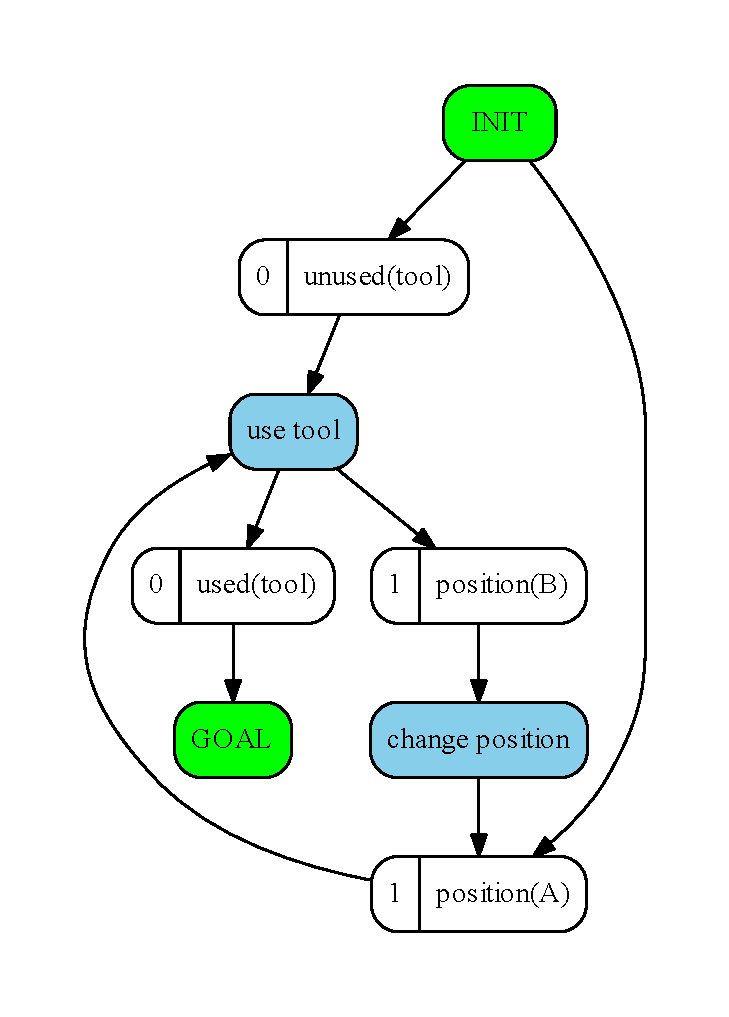
\includegraphics[scale=0.4]{oneUsage/figures/startsInInit_input}
			\caption{before reduction}
		\end{subfigure}	
		\begin{subfigure}[b]{0.4\textwidth}
			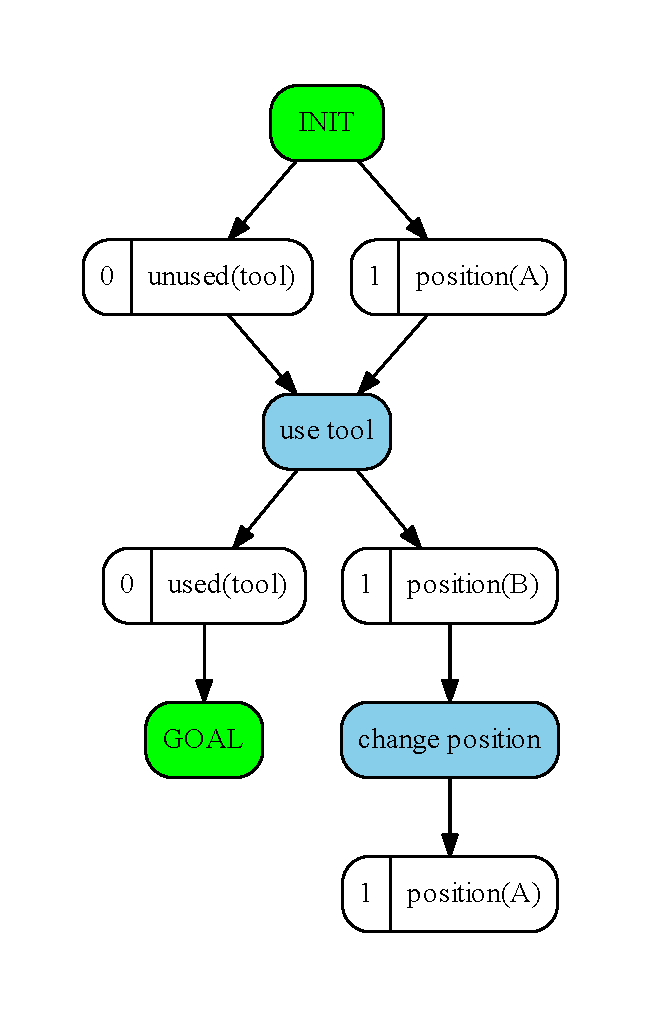
\includegraphics[scale=0.4]{oneUsage/figures/startsInInit_output}
			\caption{after reduction}
		\end{subfigure}
		\caption{case A: $w_i \in \init$; $\var{w_j} = $ variable 1, $\var{u_j}$ = variable 0, $a_c$ = \emph{use tool}, $a_d = $ \emph{change position}, $w_i = $ \emph{1 position B}}
	\end{figure}
	
	
	Case B: $w_j \in \init$
	
	\begin{enumerate}
		\item $\dom{\var{w_i}} = \dom{\var{w_i}} \cup \{w_n\}$
		\item $a_c' \leftarrow <\pre{a_c},(\eff{a_c} \setminus \{<w_i,w_j>\}) \cup \{<w_i,w_n>\}>$, 
		\item $\actions{}' \leftarrow (\actions \setminus \{a_c\}) \cup \{a_c'\}$ 
	\end{enumerate}		
	
	
	\begin{figure}
		\begin{subfigure}[b]{0.4\textwidth}
			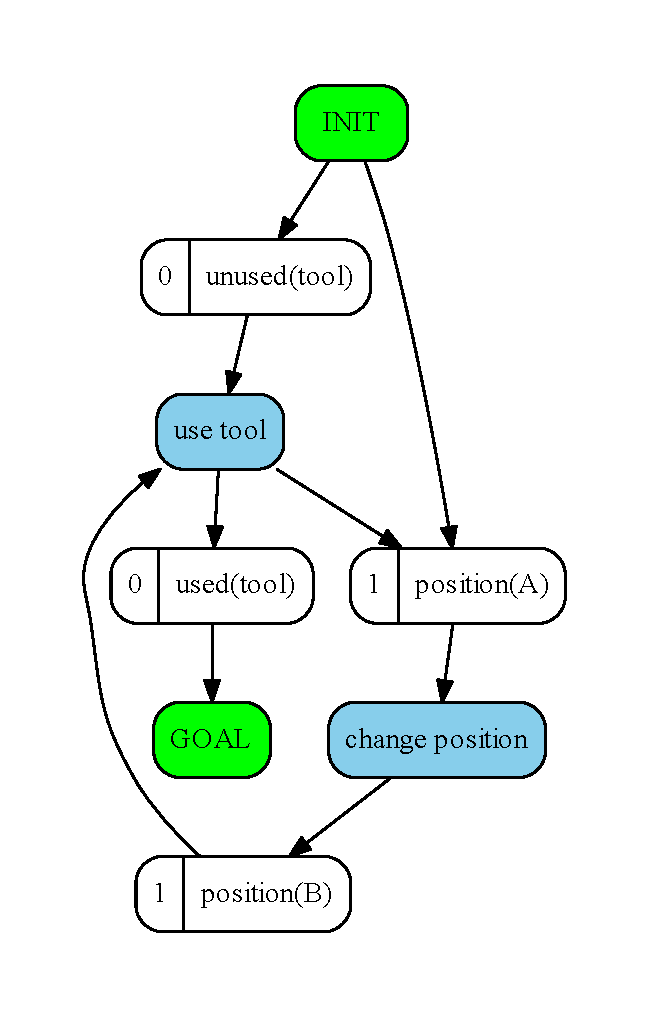
\includegraphics[scale=0.4]{oneUsage/figures/endsInInit_input}
			\caption{before reduction}
		\end{subfigure}	
		\begin{subfigure}[b]{0.4\textwidth}
			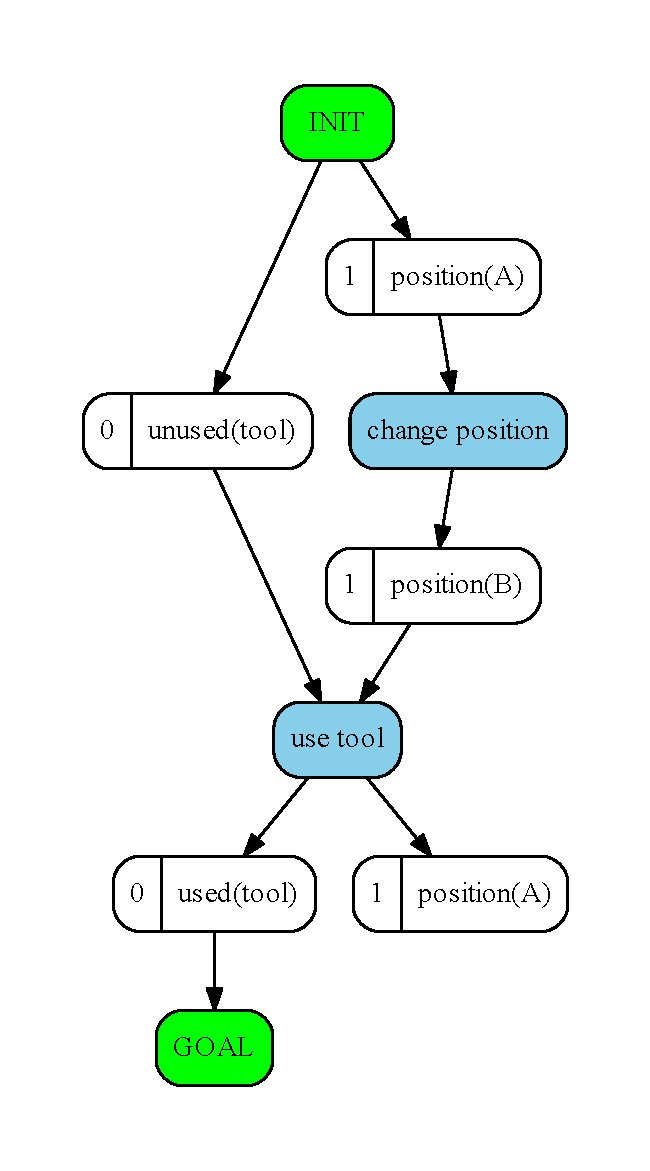
\includegraphics[scale=0.4]{oneUsage/figures/endsInInit_output}
			\caption{after reduction}
		\end{subfigure}
		\caption{case B: $w_j \in \init$; $\var{w_j} = $ variable 1, $\var{u_j}$ = variable 0, $a_c$ = \emph{use tool}, $a_d = $ \emph{change position}, $w_j = $ \emph{1 position A}}		
	\end{figure}
	
	
	Output of the reduction is SAS $<\vars{}', \init{}, \goal{}, \actions{}', \mutexes{}>$.
	
	
	\section{Possible outgoing states of SAS}
	\begin{enumerate}
		\item application of -oe, -sf, -ai
	\end{enumerate}
	
	After implementing this reduction, other reduction were implemented; namely -sf or -ai could be doing some operation with the SAS that this reduction may become redundant in some cases.
	
	\section{States before application of this operation}
	\begin{itemize}
		\item from the beginning
		\item after application of -sd, -hc, -mo, maybe others (does not which right now)
	\end{itemize}
	
	
	\section{Reverse operation}
	During the reverse operation, effect of type $<w_i,w_n>$ are replaced back by $<w_i,w_j>$ and $<w_j,w_n>$ are replaced back by $<w_j,w_i>$. No extension of the plan is done.
	
	\section{Implementation notes}
	Now, it returns multi reverse operation.
	
	There is some bug. Only thing I came up with is that in current implementation, there are no such strict condition over set of consumers and producers. If the bug is not hidden inside these condition, then I would revise method Operation.isProducing(value) if the -1 value is used without mistakes. There is also possibility that implementation does not contain check for $w_i$ or $w_j$ to be in $\init$.
	
	The name of newly added fact is quite unimportant. In the implementation, there the name is get as copy of the fact that is being replaced. This is because preprocess of FD is parsing names of facts (so it cares about predicate names, etc, somehow). Also it should be run before -uv.
	
	
	\chapter{Generalized actions -ga}

	Suppose that there is a variable having two values $u_i, u_j$ and there are two actions that differs only in one thing. The difference is that one action has got $u_i$ in prevail precondition and the second has got $u_j$ in its prevail precondition. In such scenario, both actions can be generalized into one - the generalized action does not have any precondition on variable $\var{u_i}$. By this, we can reduce number of actions.


	\begin{figure}
		\begin{subfigure}[b]{0.8\textwidth}
			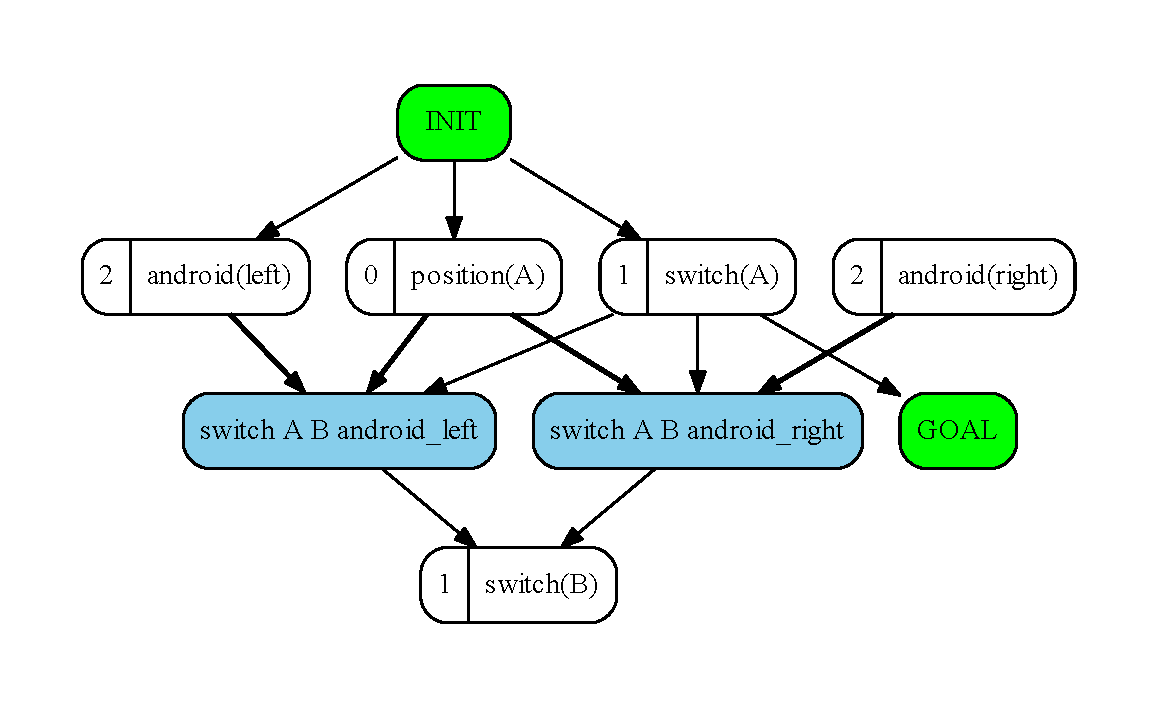
\includegraphics[scale=0.5]{generalizeActions/figures/simple_input}
			\caption{before reduction}
		\end{subfigure}	
		
		\begin{subfigure}[b]{0.8\textwidth}
			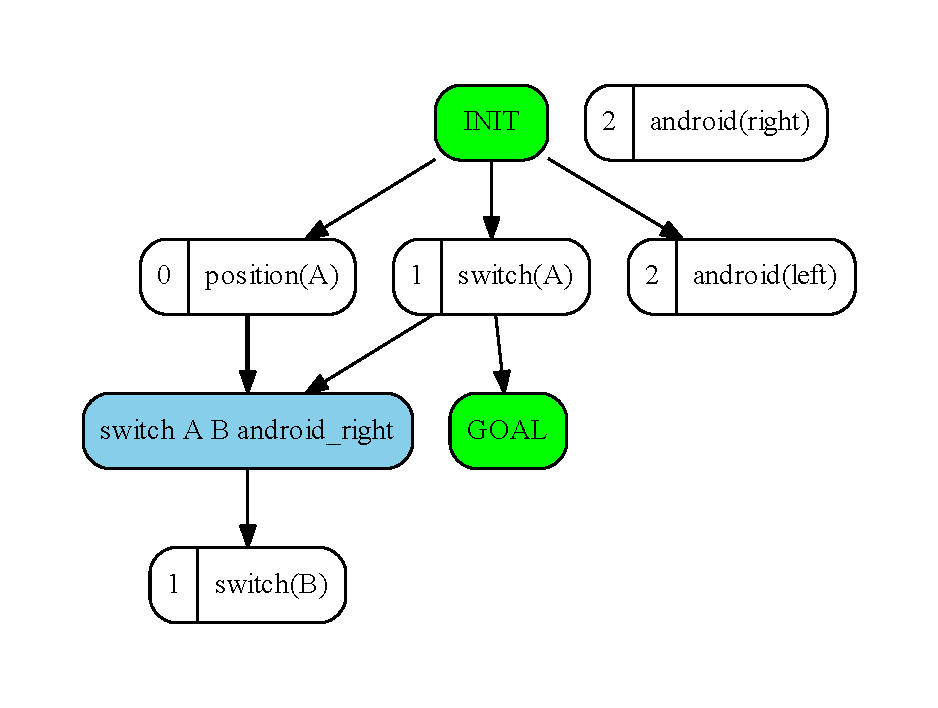
\includegraphics[scale=0.5]{generalizeActions/figures/simple_output}
			\caption{after reduction}
		\end{subfigure}
		\caption{Both action from the example can be generalized because their together cover all possibilities of variable 2 in preconditions. }
	\end{figure}               
	
	
	\section{Reduce operation}
	Let's have SAS in form $<\vars, \init, \goal, \actions, \mutexes{}>$. Suppose that we an action $a$. Then for each variable $v$ there exists set of actions $A_d$ that is created in this way: $\exists v \in \vars: A_v \leftarrow \{<\pre{a} \cup \{u\},\eff{a}> | \forall u \in \dom{v} \} $.
	
	If 	$A_v \subseteq \actions$ is satisfied for arbitrary $v$, then this operation can be executed. Then $a$ is generalized action thanks to variable $v$. 
	
	Now, the reduction can be executed as follow:
	
	\textbf{Case A)} $a \in \actions$
	$\actions{}' \leftarrow \actions \setminus A_s$
	
	\textbf{Case B)}
	$\actions{}' \leftarrow (\actions \setminus A_s) \cup \{a\}$
	
		
	Output of the reduction is SAS $<\vars{}, \init{}, \goal{}, \actions{}', \mutexes{}>$.
	
	
	\section{Possible outgoing states of SAS}
	\begin{enumerate}
		\item states of SAS where -mv, -bv, -uv, -mo, -sd, -hc can be executed, maybe also others
	\end{enumerate}
	
	\section{States before application of this operation}
	\begin{itemize}
		\item original SAS
		\item after execution of -dv, -mv
	\end{itemize}
	
	
	\section{Reverse operation}
	\textbf{Case A)} Removed actions are added back to SAS. No extension of the plan is done, because original SAS already contained generalized actions, so removed actions were redundant.
	
	\textbf{Case B)} Removed actions are added back to SAS. The plan is simulated and when action $a$ is used in the plan, it is replaced by corresponding action from $A_v$ having current value of variable $v$ in its prevail preconditions.
	
	
	\section{Implementation notes}
	Current implementation returns MultiReverseOperation.		
	\chapter{Use applicable action in start -ai}

Aim of this operation is to find actions that are applicable in init, do not destroy possibility of applying another action and can be used at most once; once such action is found, is applied to init and removed from SAS. 

\begin{figure}
	\begin{subfigure}[b]{0.4\textwidth}
		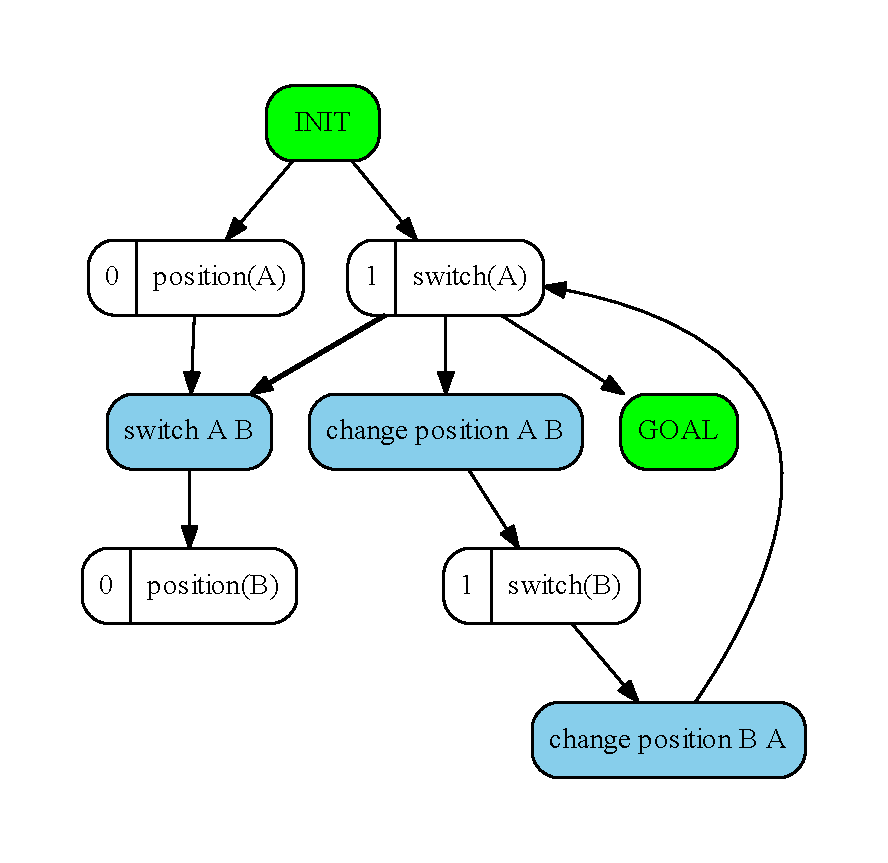
\includegraphics[scale=0.4]{useApplicableActionInStart/figures/applyOnlyOne_input}
		\caption{before reduction}
	\end{subfigure}	
	\begin{subfigure}[b]{0.4\textwidth}
		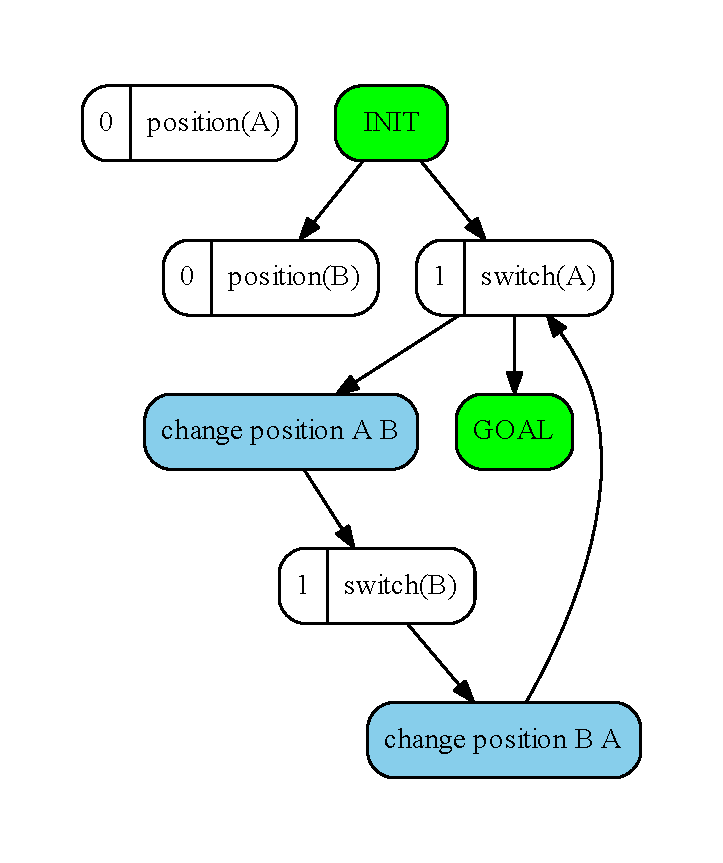
\includegraphics[scale=0.4]{useApplicableActionInStart/figures/applyOnlyOne_output}
		\caption{after reduction}
	\end{subfigure}
	\caption{Action \emph{switch A B} can be applied in init, is applicable at most once and does not destroy application of other actions. Action \emph{change B A} is not applicable in init. Action \emph{changes A B} is applicable in init but it may be applied more than once and its application destroys usage of \emph{switch A B}.}		
\end{figure}


\section{Reduce operation}
Let's have SAS in form $<\vars, \init, \goal, \actions, \mutexes{}>$. 

This operation is executed if there is action $a$ such that:

\begin{enumerate}
	\item $a$ is applicable in init; $\pre{a} \subseteq \init, \del{a} \subseteq \init$
	\item $a$ is applicable at most once; $\forall \todo{$\exists$ ?} u \in \del{a}: |\pro{u}| = 0$
	\item $a$ does not destroy application of any other action ; $\forall u \in \del{a}: |\wan{u}| = 1$	
\end{enumerate}

Note, the last condition also says that there must not be any effect of type $<-1,u_j>$ where $u_j \in \dom{\var{u}}$.

The reduction operation does following things:
\begin{enumerate}
	\item apply $a$ on init; $\init{}' \leftarrow (\init \setminus \del{a}) \cup \{\add{a}\}$
	\item remove $a$ from actions; $\actions{}' \leftarrow \actions \setminus \{a\}$
\end{enumerate}	


Output of the reduction is SAS $<\vars{}, \init{}', \goal{}, \actions{}', \mutexes{}>$.


\section{Possible outgoing states of SAS}
\begin{enumerate}
	\item application of -uv, -oe, -ou, -sf, -ai
	\item note that values removed from init could be removed from SAS but in current implementation they are not, so they are removed after executing -uv
\end{enumerate}


\section{States before application of this operation}
\begin{itemize}
	\item from the beginning
	\item after execution of -mv, -bv, -oe, -ou, -sf, -ga
\end{itemize}


\section{Reverse operation}
Removed things are added back to the SAS. Action $a$ is added at the first position to the given plan and such extended plan is returned.


\section{Implementation notes}
Now, it returns multi reverse operation.


	\chapter{Single first action merge with start -sf}
	
If there is only one action that is applicable in start and goal is not subset of init, then such action can be executed because there is no other possibility to get from init to goal. While -ai removes applied action from SAS, this reduction does not removes applied action. 

Please TODO.
		\chapter{Action start merge -as}
	Suppose we have action $a$ that can be executed in init and can be executed at most once. Such action holds an invariant effect of type $<u_i,u_j>$ where $u_j$ is not used in any other action. But if we know that $a$ has invariant effect $<u_i,u_j>$ and also effect $<w_i,w_j>$ so then, there could be invariant effect $<w_j,w_i>$ in other actions. If there are such a link, then action $a$ is applied - this is what this operation does.
	
	But in implementation (as in older text here) are some mistakes. Firstly, $a$ can have prevails preconditions but they have to be satisfied by init.
	
	\textbf{Another mistake} written here and already implemented is that there is no check whether action $a$ does not destroy usage of other actions. So, there should be or - either effect in $a$ in the is invariant, invariant together with another action (there is the cycle) or it deletes something that is not used in any other function (not in delete effect nor prevail preconditions).
	
	Also, this operation seems to be old, because after implementing -sf, -ai, -ou and -oe these reduction may have the same effect as this one. Suppose that firstly -ou removes replaces invariant by new one (by adding new fact), then if -ai or -sf is applied, the action $a$ can be merged with start.
	
	\begin{figure}
		\begin{subfigure}[b]{0.4\textwidth}
			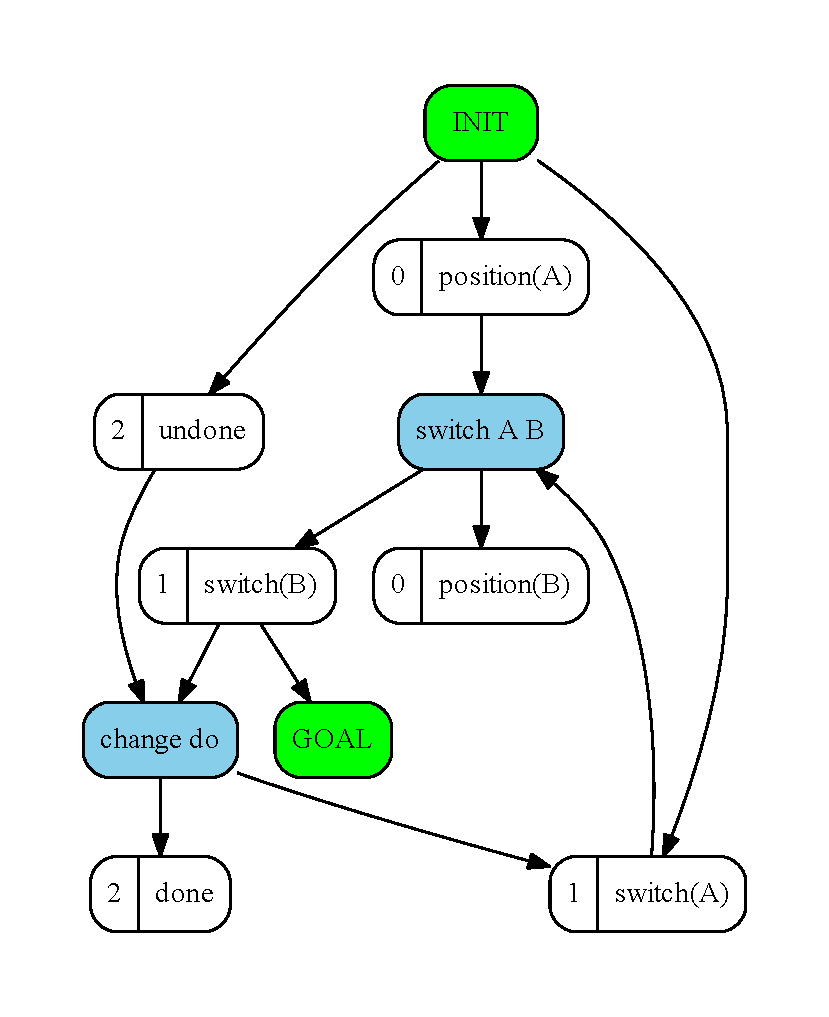
\includegraphics[scale=0.4]{actionStartMerge/figures/simple_input}
			\caption{before reduction}
		\end{subfigure}	
		\begin{subfigure}[b]{0.4\textwidth}
			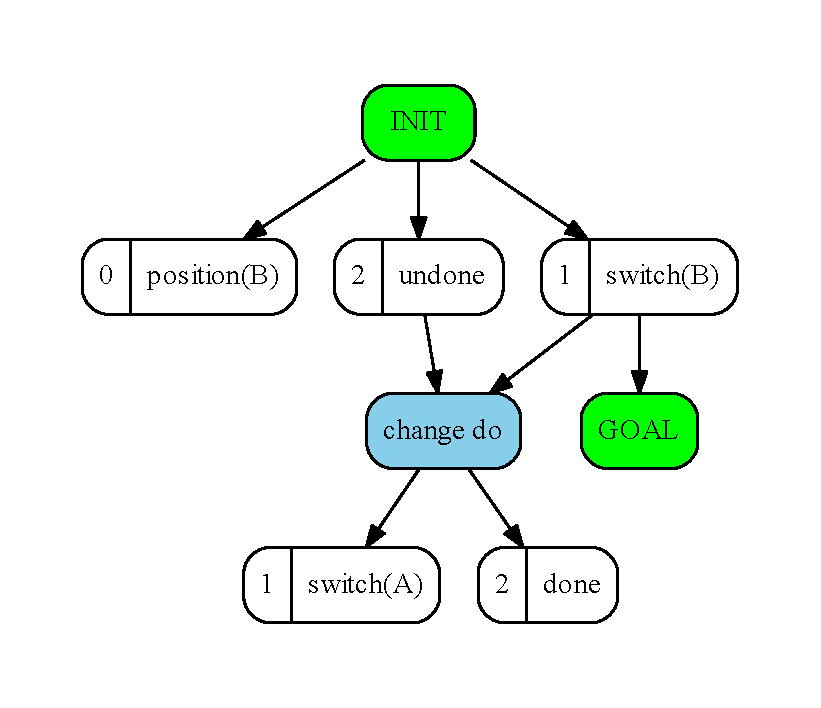
\includegraphics[scale=0.4]{actionStartMerge/figures/simple_output}
			\caption{after reduction}
		\end{subfigure}
		\caption{Action \emph{switch A B} was applied because it is applicable in init, it can be used at most once ($<\emph{0 position(A), 0 position(B)}>$). Since this action can be applied at most once, then \emph{change do} can be also applied at most once. So, \emph{switch A B} can be merged with start because it will not destroy application of any other function.	}
	\end{figure}
	
	\section{Reduce operation}
	Let's have SAS in form $<\vars, \init, \goal, \actions, \mutexes{}>$. There must be following values and actions in order to execute the action:
	
	\begin{enumerate}
		\item $a \in \actions$
		\item $|\pre{a}| = 0$ - such is implementation, $\pre{a} \subseteq{\init}$ is better 
		\item $<u_i,u_j> \in \eff{a}$
		\item $u_i \in \init$, $|\con{u_i}| = 1$
		\item $|\con{u_j}| = 0$
		\item $\forall <w_i, w_j> \in \eff{a}, \var{w_i} \neq \var{v_i}:$
		\begin{itemize}
			\item $w_i \in \init$
			\item $ \forall a_p \in \pro{w_i}: <w_j,w_i> \in a_p $ 
			\item $ \forall a_c \in \con{w_j}: <w_j,w_i> \in a_c $ 
		\end{itemize}
	\end{enumerate}
	
	Such effect $<u_i, u_j>$ with condition over $u_i$ and $u_j$ ensures that $a$ can be executed only once and in init. For each different effect than $<u_i,u_j>$, let say $<w_i,w_j>$, there must hold that all action consuming $w_j$ also contains effect $<w_j,w_i>$ and that there are only one action that needs $w_i$ (action $a$).
	
	The operation does following things:
	
	\begin{enumerate}
		\item for each effect $e \in \eff{a}$, $e = <w_i, w_j>$; do: $u_i$ is replaced by $u_j$ in $\init$, $u_i$ is replaced by $u_j$ in mutexes and in init
		\item remove $u_i$ from $\dom{\var{u_i}}$
		\item final init is stored in $\init{}'$
		\item $\actions{}' \leftarrow \actions \setminus \{a\}$
		\item for each effect $<w_i,w_j> \in \eff{a}, \var{w_i} \neq \var{u_i}$ do following things
		\begin{enumerate}
			\item $\actions{}'  \leftarrow \actions$
			\item for each $a_p \in \pro{w_i} \cup \con{w_j}$ do following
			\item $a_n \leftarrow <\pre{a_p} \cup{w_j}, \eff{a_p} \setminus \{<w_i,w_j>,<w_j,w_i>\} >$
			\item if $|\eff{a_p}| > 0$ $\actions{}' \leftarrow (\actions{}' \setminus \{a_p\}) \cup \{a_n\}$
			\item else $\actions{}' \leftarrow \actions{}' \setminus \{a_p\}$ 
		\end{enumerate}
	\end{enumerate}
	
	Output of the reduction is SAS $<\vars{}', \init{}', \goal{}, \actions{}', \mutexes{}'>$.
	
	
	\section{Possible outgoing states of SAS}
	\begin{enumerate}
		\item possible empty mutex
		\item possible state of SAS for delete variable -dv, merging actions -mo, simple dependency -sd, maybe even one usage reduction -ou and action start merge -as, -sf, -ai
	\end{enumerate}
	
	\section{States before application of this operation}
	\begin{itemize}
		\item SAS from beginning
		\item after -mo, -ou, -dv
		\item maybe after -oe, -as, -ai, -sf
	\end{itemize}
	
	
	\section{Reverse operation}
	Removed actions and values are added back and added actions $a_n$ are removed from the action set. Action $a$ is added at the first position in the plan and such extended plan is returned.
	
	\section{Implementation notes}
	Simple implementation without any advance caching. There may be speed up by comparing set $\con{w_j} = \pro{w_i}$, if they equal. Now, the implementation is done as written above - for each effect, it check if all consumers and producers have got the right effect.
	
	
	

		\chapter{Check -ch}
	This is not reduction operation. In fact, it is a function that stops executing reductions if they are not needed. 
	
	Let have SAS in form $<\vars, \init, \goal, \actions, \mutexes{}>$. If $\goal \subseteq \init$ then stop further reductions; otherwise continue.
	
	If the check is set to true, then it tests if $\goal \subseteq \init$ after each reduction.
			
	
\end{document}
